\section{Results: Adaptation Budget and Drift (RQ2)}
\label{sec:res_budget}

\begin{figure}[t]
  \centering
  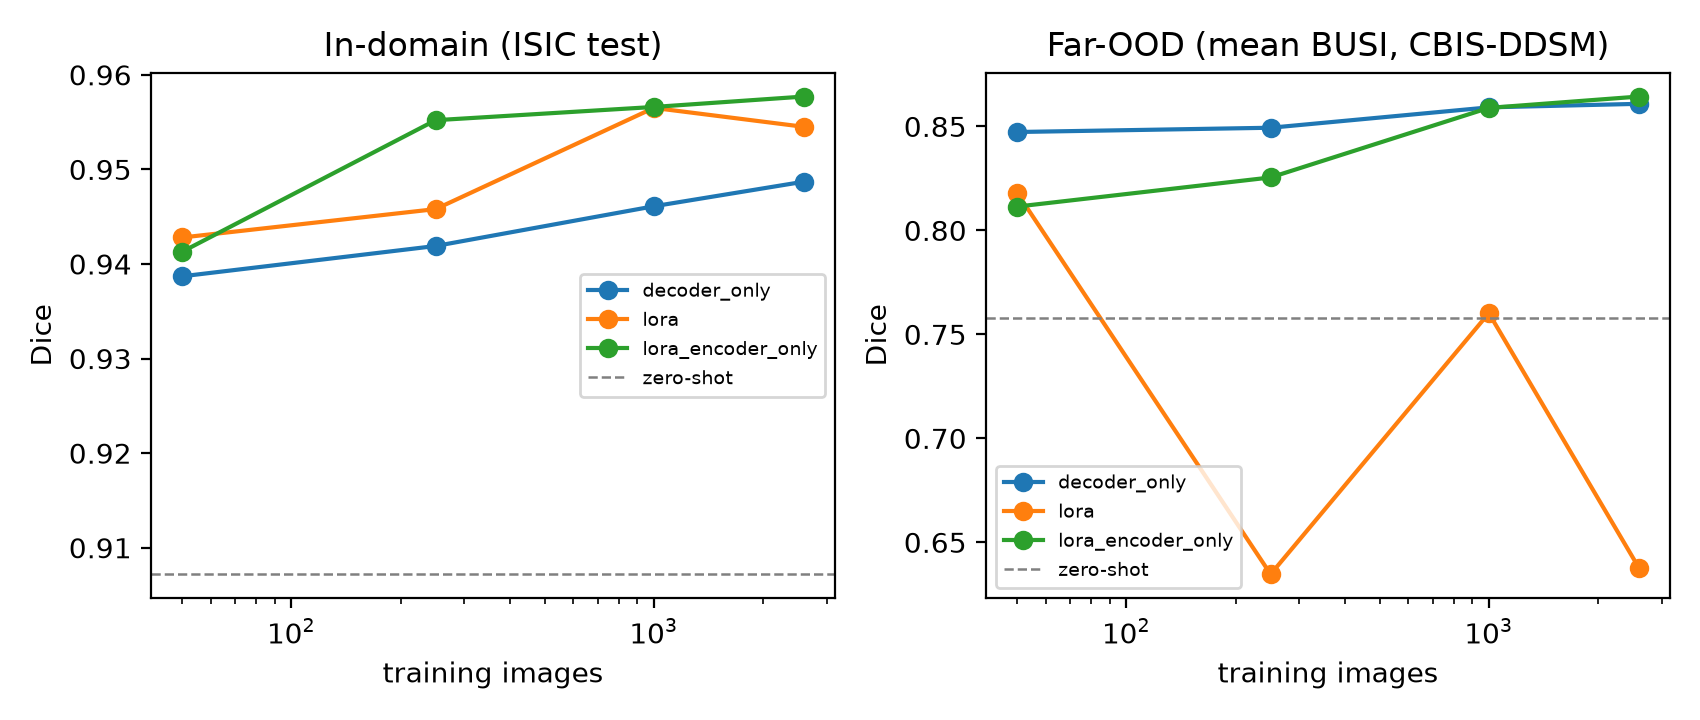
\includegraphics[width=0.74\linewidth]{figures/budget_curves.png}
  \caption{Adapters trained for 6000 steps on nested subsets (log axis), zero-shot dashed. Left: in-domain Dice. Centre: far-OOD Dice (mean of BUSI, CBIS-DDSM). Right: far-OOD drift ($1 - \mathrm{CKA}$ to the base) of the decoder's upscaled embedding (circles) and encoder neck (squares, dashed). Dice: mean and std over three seeds at 50 to 1000 images; the 2595-image point and the drift panel are seed 0.}
  \label{fig:budget}
\end{figure}

\paragraph{The collapse appears at 250 images, with decoder drift.}
Decoder-only fine-tuning and encoder-only LoRA improve on both axes of Fig.~\ref{fig:budget} at every budget and stay above the zero-shot far-OOD reference of 0.758 in every seed. LoRA with a trainable decoder is the only method that crosses it: $0.790 \pm 0.027$ at 50 images, $0.670 \pm 0.031$ at 250 (below zero-shot in all three seeds), $0.774 \pm 0.019$ at 1000 and 0.638 with all 2595 images, while its in-domain Dice rises monotonically. Its far-OOD decoder drift triples between 50 and 250 images, from 0.12 to 0.36, where its Dice collapses, and stays there; the partial recovery at 1000 images occurs at unchanged drift, so drift marks the onset of the collapse rather than its depth. Decoder-only fine-tuning retrains every decoder weight yet keeps far-OOD decoder drift below 0.06, and encoder-only LoRA moves the encoder twice as much as LoRA (encoder drift 0.25 against 0.12) while keeping decoder drift below 0.09. Neither little data, decoder training nor encoder movement alone causes the collapse.

\paragraph{Controls: rank, decoder and learning rate.}
Encoder-only LoRA differs from LoRA in rank and target layers as well as in the frozen decoder, and LoRA's decoder trains at $5 \times 10^{-4}$ against $10^{-4}$ in decoder-only fine-tuning. Rank-8 query-key-value LoRA with the decoder frozen reaches far-OOD Dice \pending{X.XXX $\pm$ X.XXX} (LoRA: \pending{X.XXX}), and LoRA with its decoder at $10^{-4}$ reaches \pending{X.XXX $\pm$ X.XXX} (tight boxes, full data, three seeds). \pending{Interpretation once T10 lands: if both recover, the collapse needs a decoder updated quickly alongside the encoder; if only the frozen-decoder run recovers, decoder training itself is the cause.} Full fine-tuning also adapts both halves but at $10^{-5}$ and does not collapse, so the evidence locates the failure in joint encoder--decoder adaptation at PEFT learning rates, not in joint adaptation as such.
